% Letting the Tools Do the Math -- submission to TMLR.
% Build in this folder: tectonic paper.tex

\documentclass[10pt]{article}

% SUBMISSION: plain \usepackage{tmlr} -> "Anonymous authors", "Under review as submission to TMLR".
% arXiv: [preprint] (names shown, no TMLR header) -- tools/paper/check_paper.py --preprint builds
% that variant from this file, so there is one source. Camera-ready: [accepted], which also needs
% \month, \year and \openreview defined (see the TMLR template).
\usepackage{tmlr}
\usepackage{microtype}
\usepackage{graphicx}
\usepackage{booktabs}
\usepackage{array}
\usepackage{amsmath}
\usepackage{hyperref}
\usepackage{xurl}
\usepackage{etoolbox}
\graphicspath{{figures/}}
% The preprint prints no running head; drop the rule that would sit empty above it.
\makeatletter\if@preprint\renewcommand{\headrulewidth}{0pt}\fi\makeatother

% Links as blue text without boxes, as in the author's other paper.
\hypersetup{colorlinks=true, linkcolor=blue, citecolor=blue, urlcolor=blue}
% Table captions sit above their tables, so the space goes below the caption, not above it
% (tmlr.sty keeps LaTeX's defaults, which put the table's top rule against the caption).
\AtBeginEnvironment{table}{\setlength{\abovecaptionskip}{0pt}\setlength{\belowcaptionskip}{6pt}}

\newcommand{\tok}[1]{\texttt{\small #1}}

% DEANONYMIZED is true in the [preprint] (arXiv) and [accepted] builds -- tmlr.sty sets @accepted in
% both -- and false in the submission. The TMLR template: author contributions and acknowledgments
% go in "only once your submission is accepted and deanonymized".
\makeatletter
\newif\ifdeanonymized
\if@accepted\deanonymizedtrue\else\deanonymizedfalse\fi
\makeatother
% The review copy says "the authors", as its header does ("Anonymous authors").
\newcommand{\theauthor}{\ifdeanonymized the author\else the authors\fi}
\newcommand{\Theauthor}{\ifdeanonymized The author\else The authors\fi}

% Explicit breaks: tmlr.sty sets the title justified in \LARGE sans, which hyphenated "Calcula-tor".
\title{Letting the Tools Do the Math:\\A 10.9M-Parameter Language Model\\on a Graphing Calculator}

% Hidden by tmlr.sty in the submission build; printed in [preprint] and [accepted].
\author{\name Alexander Messerlian \email alex.messerlian@icloud.com\\
      \addr Independent Researcher, Palo Alto, CA, USA}

\begin{document}

\maketitle

\begin{abstract}
We built a physics assistant that runs entirely on a TI-Nspire CX II CAS graphing calculator: one
ARM926EJ-S core at 396\,MHz, no floating-point unit, a largest single memory allocation of about
21.5\,MiB and no network.\footnote{AI tools wrote most of the software and experiment tooling and
drafted the text; the Statements and Declarations after the conclusion describe their roles.
Responsibility for the content lies with \theauthor.} We use it as a case study in how the
conclusions of a small-model evaluation depend on what the evaluation runs. The 10.9M-parameter
model never computes: the runtime picks a relation from a store, puts it in the prompt with the
question's values, and runs the tool call the model writes. Given the right relation, the model is
right on 96.7\% of problems that give every value; its errors are digits copied wrongly, and an
irrelevant value placed before the relevant ones lowers its score from 116 to 61 of 120, a pattern
consistent with the training generator's habit of adding irrelevant values last. End to end, on
generated problems, choosing the relation was at first the main limit: the system answered 21 of the
same 120 problems correctly and declined most of the rest. Two selection rules that use the values
the question assigns raise this to 93 (and to 248 of 300 fresh problems from the same generators),
while wrong answers rise from 2 to 4. A rule-based path through the same runtime with no model is
right more often and wrong less often on every set that asks for a number; the model declines more
reliably. Differences between our harness and the calculator moved strict accuracy by 9 to 21
points and exposed an engine defect that a host--calculator comparison could not detect. A
per-token cost model fitted on battery predicts a decode run within 0.4\%.
\end{abstract}

% ==================================================================================================
\section{Introduction}
\label{sec:intro}

This paper is a case study in how the conclusions of a small-model evaluation depend on what the
evaluation actually runs. The setting is a graphing calculator, a machine students already bring to
class. The TI-Nspire CX II CAS has one ARM926EJ-S core at 396\,MHz, no floating-point unit and no
SIMD, no network, and a largest single memory
allocation of about 21.5\,MiB. We built a physics assistant that runs on it by itself, on battery, and measured what it
costs, where it fails, and what its model contributes.

These limits push the design one way: take out of the weights everything a small model is likely to get
wrong. Arithmetic goes to an evaluator that runs on the calculator. The physics goes to a store
of 177 relations, each with its units and conditions. The runtime picks one relation and puts it in
the prompt, with the question's values and the inputs it gives no value for. The
10.9M-parameter model then only reads the prompt, copies values into a call and writes a sentence
around the result, or declines, or explains a relation.

Each time we brought our evaluation closer to the system that actually runs, its result changed. Our contributions are measurements of those steps:
\begin{itemize}
\setlength{\itemsep}{1pt}
\item how the prompt text, the decoding method and the calculator's int8 engine each moved
  measured strict accuracy, by 9 to 21 points, including an engine defect that a host--calculator comparison could not
  detect, found only by scoring on the calculator's decoder and fixed at a 2.3\% speed cost
  (Section~\ref{sec:eval});
\item with the right relation supplied, what errors the model makes: copying mistakes, and a
  sensitivity to where an irrelevant value is placed; and a baseline with no model that, with the
  relation supplied, matches or beats the model on every number and refusal (Section~\ref{sec:quality});
\item in the full system, with the application choosing the relation: where accuracy was lost,
  counted as right, wrong and declined, with a repeat on fresh problems, a negative set whose values bind a relation that does
  not apply, and the no-model baseline behind the same selector (Section~\ref{sec:e2e});
\item a model of the cost of one token by depth, width and position, fitted on battery, and the
  limits that memory and speed set on model size; an empty KV cache (the stored keys and values of earlier positions)
  understates the cost of each added position by 40\% (Sections~\ref{sec:cost}
  and~\ref{sec:frontier}).
\end{itemize}
The assistant itself, in which the model never computes, is the setting (Section~\ref{sec:arch});
Appendix~\ref{app:ladder} compares two model widths, with two seeds each.

% ==================================================================================================
\section{Related Work}
\label{sec:related}

\textbf{Language models on graphing calculators.} We know of three earlier projects, all released
in July and August 2026 (Table~\ref{tab:prior}): CalcGPT~3 \citep{fredbennett2026calcgpt}; Transformer
On Calc, the closest in method, which runs a 260K-parameter llama2.c model natively on the same
calculator \citep{stepney141transformeroncalc}; and CasioLLM, which streams a quantized model of up
to 25M parameters from flash on a Casio fx-CG50 without a third-party loader
\citep{samilososami2026casiollm}. We describe them rather than benchmark them, because none measures
the same thing: none uses tools or retrieval, and none reports a cost model or a measured memory limit. A
TI-84 modification that sends questions over Wi-Fi to a cloud model is different in kind, since no
model runs on the calculator \citep{chromalock2024ti32}.

\begin{table}[t]
\caption{Language models that run on graphing calculators, as their authors describe them. Timings
cannot be compared across rows: the workloads, vocabularies and timing methods differ, and only this
work states the power state.}
\label{tab:prior}
\centering\small
\setlength{\tabcolsep}{4pt}
\newcolumntype{L}[1]{>{\raggedright\arraybackslash}p{#1}}
\begin{tabular}{@{}L{2.2cm}L{2.5cm}L{2.3cm}L{2.0cm}L{3.1cm}L{3.0cm}@{}}
\toprule
 & device & how it runs & weights & model & timing reported \\
\midrule
CalcGPT 3 & TI-Nspire & built-in Python & not stated & 8-bit GRU, 640-word vocabulary, dialogue & none \\
Transformer On Calc & TI-Nspire CX II CAS & native, Ndless & not stated & 260K llama2.c, TinyStories & ${\sim}9$ (fp32) / ${\sim}16$ (int8) tok/s, 64 tokens \\
CasioLLM & Casio fx-CG50 & native add-in & streamed from flash & third-party, up to 25M, 4-bit & 10-token reply in 27.1\,s \\
This work & TI-Nspire CX II CAS & native, Ndless-derived & in RAM & 10.9M, int8, trained here; tools & 1.88 tok/s decode at positions 53--87; 26--75\,s per turn from the start of generation; battery \\
\bottomrule
\end{tabular}
\end{table}

\textbf{Tool use and program-aided reasoning.} Letting a model call a tool instead of computing is
well established. Toolformer learns when to call an API \citep{schick2023toolformer}; PAL and
Program of Thoughts write programs for an interpreter to run \citep{gao2022program,chen2022program};
Calc-X, ArithmeticGPT, MathSensei and OccamLLM focus on arithmetic
\citep{kadlcik2023calcx,liu2025arithmeticgpt,das2024mathsensei,dugan2024occamllm}; and T1 shows small
models gaining from handing verification to tools \citep{kang2025tool}. Retrieval-augmented
generation supplies knowledge the weights lack \citep{lewis2020retrieval}, and picking the right tool
from a large collection limits later success in ways that a benchmark which supplies the tool hides
\citep{shi2025retrieval}. Our selector picks one physics relation with fixed rules rather than
retrieving from a large tool set, but comparing a supplied relation with a selected one, as
Section~\ref{sec:e2e} does, is the same measurement. Tool use is therefore not our contribution, and
neither is the observation that tool-augmented models fail in recognizable ways
\citep{trevino2025benchmarking} or that irrelevant information in a problem misleads language models
\citep{shi2023large}. What differs is the setting, a 10.9M-parameter model on hardware with no FPU
and no network, and what can be measured there: with the arithmetic handed off, which errors remain,
and how they relate to the training data.

\textbf{Small models and scale.} TinyStories showed that models of a few million parameters can
write fluent text in a narrow domain \citep{eldan2023tinystories}, and MobileLLM studies design
choices below a billion parameters \citep{liu2024mobilellm}. Scaling laws relate loss to parameters
and data \citep{kaplan2020scaling,hoffmann2022training}. Our comparison of two
widths asks a narrower question, with data and training steps held fixed: which behaviors a
3.5-fold reduction in parameters removes.

\textbf{Inference under tight budgets.} Work on microcontrollers fits networks into kilobytes to
megabytes \citep{lin2020mcunet,lai2018cmsis}, including small language models
\citep{scherer2024deeploy,yang2024mcubert}, and microcontrollers have served as tool endpoints for a
model hosted elsewhere \citep{yang2026device}. We use integer quantization with a scale per group
\citep{jacob2017quantization,dettmers2022matrix}. Streaming weights from flash
\citep{alizadeh2023flash}, as CasioLLM does, avoids a RAM limit at a cost in speed; we keep the
weights in memory and discuss the trade-off in Section~\ref{sec:frontier}. Our cost model has the
same aim as the roofline model \citep{williams2009roofline}, but it is fitted to measurements on the
device rather than derived from peak rates.

\textbf{Evaluation fidelity.} That a model's evaluation path and its serving path must compute the
same values is standard production practice: the ML Test Score asks for a test that training and
serving features are identical \citep{breck2017mltestscore}, deployed models are known to differ from their reference implementations \citep{qiu2022mlexray}, and inference engines have a documented set
of bugs \citep{liu2025first}. We do not claim this mismatch is new. We measure how far each
difference moved the evaluation of one small model, and report a defect that a host--calculator
comparison cannot see, because both sides run the same code (Section~\ref{sec:defect}).

% ==================================================================================================
\section{System}
\label{sec:arch}

\subsection{The model never computes}

A question passes through four steps (Figure~\ref{fig:exchange}).

\textbf{Selection.} The runtime ranks the store's 177 relations, together with 1,442 glossary terms
from the same textbooks (Section~\ref{sec:data}), against the question, and acts only when it is
confident. It is confident when the question writes out a stored relation, or under three rules.
The \emph{coverage rule}: the name of the top-ranked relation covers at least three quarters of the
question's content words. The \emph{values rule}: the values the question assigns bind the
top-ranked relation, supplying exactly its inputs, and bind no other. The \emph{asked-symbol rule}:
among the relations those values bind, exactly one computes the symbol the question asks for.
Otherwise it picks nothing, the prompt says that no relation matched, and the model declines.
Section~\ref{sec:e2e} measures this step and explains where the last two
rules came from.

\textbf{Assembly.} Native code reads the values the question gives (\tok{m = 2}), moves them to the end of
the question and builds the prompt: the question, then a record holding the relation, the unit of each variable, the inputs it gives no value for (\tok{missing}), the conditions under
which the relation holds, and any physical constant it needs.

\textbf{Generation.} The model continues the prompt. When it closes a \tok{<tool>} span, the runtime
runs the call and inserts the result as a \tok{<res>} span; the model then writes its answer and
ends with \tok{<end>}. The calculator decodes greedily. If the answer states a number more than 2\% from the result, the runtime appends the
computed value.

\textbf{Execution.} The evaluator supports seven tools: \tok{eval}, \tok{evalat}, \tok{solve},
\tok{diff}, \tok{integ}, \tok{conv} and \tok{stat}. Units are handled only inside \tok{conv};
everywhere else every name is a symbol, so \tok{g} is gravity, not grams.

During training the loss is masked on every \tok{<res>} span, so the model learns to write calls and
to restate what it is given, not to predict what the evaluator will return.

\begin{figure}[t]
\centering
\fbox{\parbox{0.95\linewidth}{\small\ttfamily\raggedright
<q>Take What was the motionally induced emf? Given l = 0.057, v = 1.35, B = 0.196..</q>\\
<r>epsilon=B*l*v | epsilon:V B:T l:m v:m/s | missing:none | standard conditions | fit:high\\[3pt]
\textrm{\textit{model:}}~<tool> eval<arg> (0.196)*(0.057)*(1.35)</tool>\\
\textrm{\textit{calculator:}}~<res> 0.0150822</res>\\
\textrm{\textit{model:}}~<a> 0.01508 V. From epsilon=B*l*v.<end>
}}
\caption{A generation-and-tool turn logged on the calculator, on battery, with the relation supplied
by the test harness rather than chosen by the application's selector. From the question ``Take
l = 0.057, v = 1.35, B = 0.196. What was the motionally induced emf?'' the runtime built the prompt
(moving the values to the end, which leaves the stray ``Take'' and the double period), ran the
model's call and inserted the result. From the start of generation, including prefill (processing the
prompt), the first output appeared after 29.9\,s and the turn finished after 52.0\,s; these times exclude prompt
assembly and tokenization. The host reproduces this turn token for token
(Section~\ref{sec:parity}).}
\label{fig:exchange}
\end{figure}

\subsection{Model and tokenizer}

The model is a Llama-2-style decoder \citep{touvron2023llama} with RMSNorm \citep{zhang2019root},
rotary position embeddings \citep{su2021roformer} and a SwiGLU feed-forward block
\citep{shazeer2020variants}: width 352, six layers, eight heads, feed-forward width 1,024, a context
of 512 tokens and a vocabulary of 4,096, with the embedding shared by the output layer (the
classifier). That is 10,903,552 parameters. Weights are stored in 8 bits with one fp32 scale per
group of 88; in the file the feed-forward width is padded with zeros to 1,056 so that the group size
divides every row (Section~\ref{sec:defect}), for 11,629,696 bytes in total.

The tokenizer is trained on our corpus and reserves 11 special tokens for the document structure.
The 4,096-entry vocabulary is a speed decision: the classifier reads $\mathrm{width}\times
\mathrm{vocab}$ weights for every token, and even at 4,096 it takes 10.6\% of a token's time
(Section~\ref{sec:cost}). Scaling that measured stage linearly, we estimate that a 32,000-entry
vocabulary would add
about 0.31\,s to every token, 73\% of the current total.

Some dimensions are set by the engine rather than chosen. The group size is fixed when the engine is
compiled, because a group size read at run time costs two software divisions per group in the inner
loop, so the width must be a multiple of 88; rotary embeddings need an even head size. With eight
heads that allows widths of 176, 352 and 528, and 528 is wider
than the width-440 model that fails to load (Section~\ref{sec:frontier}).

\subsection{Engine and loader}

The inference engine is derived from llama2.c \citep{karpathy2023llama2c}. Weights are int8 with a
scale per group; before each matrix product the activations are converted to int8 per group, and the
product is summed in 32-bit integers. Normalization, rotary embeddings, attention and softmax run in
fp32 using the compiler's software floating-point routines, and the KV cache is fp32. The generation
loop, tool execution and the 2\% answer check are one C module, shared by the application and by the
evaluation harness of Section~\ref{sec:eval}. The calculator's operating system does not run native
programs, so the application is started by a loader derived from Ndless \citep{ndless}, which a
setup document installs again after every reset; the hardware is not modified (Appendix~\ref{app:device}).

% ==================================================================================================
\section{Training Data}
\label{sec:data}

The model is trained from scratch on a mixture that is, by tokens, 85\% synthetic
documents and 15\% raw textbook text. The textbook text is every module of 24 OpenStax textbooks \citep{openstax}, markup removed; 22 of the books are licensed CC BY-NC-SA 4.0 and 2 CC BY 4.0. No other dataset is used.

The synthetic documents are generated by a program from the record store, whose 177 relations were
extracted from the same books and cleaned in passes that removed malformed and non-physics records.
Each document is one exchange in the format of Figure~\ref{fig:exchange}. The generator draws each variable's value from a range chosen for that quantity, runs the call with the calculator's evaluator,
and writes the answer from a small set of templates, so the result in every document is the
evaluator's own output. Document types cover answering, declining because a value is missing,
declining because no relation matched or because the record does not apply, explaining a relation,
defining a term from the books' glossaries, and symbolic calls. The current version of the corpus
has 316,219 documents; the shipped model was trained on an earlier version from the same generator,
and the models of Appendix~\ref{app:ladder} on the current one. A check of 400 documents
sampled from an earlier 29,982-document version found 12 with a defect as a physics problem, such as mutually inconsistent values or a wrong choice
between answering and declining (3.00\%, 95\% Wilson interval 1.72--5.17\%). The check was done by two AI reading passes whose flags were settled by a further AI
pass, not by a person; its false-positive and false-negative rates were not measured, so the
interval reflects sampling uncertainty only, and the check predates later fixes, so it does not
describe the current version.

One part was produced differently. The explanation documents, one per relation (177 in training),
were drafted by an AI model, based on the relation's OpenStax section for 127 of the 177 relations
and with no source section for the other 50, and then corrected by automated checking passes that
were themselves AI-assisted. They were not written, edited or reviewed by \theauthor, and no person
has measured their error rate after correction; before correction the drafts contained a physics
error 13.4\% of the time.

Training runs 8,000 steps at batch 24 and sequence length 512 (98.3M tokens), with AdamW
(learning rate $3\times10^{-4}$, 3\% warm-up, cosine decay to 10\%, weight decay 0.1) on one laptop
GPU. The final training loss is 0.796.

% ==================================================================================================
\section{Evaluating on the Calculator's Own Code}
\label{sec:eval}

\textbf{Device and power.} Every timing in this paper is taken on one TI-Nspire CX II CAS running
OS 6.4.0.74, on battery with the USB cable unplugged: with the cable attached the core runs at
288\,MHz instead of 396\,MHz. Each measuring program reads the clock setting from the PLL and marks a run
with the cable attached as invalid. Time is read from a 32.768\,kHz crystal timer,
which does not depend on the CPU clock.

\textbf{Host scoring.} Quality is scored on a workstation, because one answer takes the calculator up
to 75 seconds. Nothing in the scoring path is rewritten for the host. The prompt is built by the
calculator's own C code for reading the question and assembling the record, and in
Section~\ref{sec:e2e} by its selection code too. Generation runs the calculator's int8 engine and
generation loop compiled for the host (together, the calculator's decoder; Apple clang 21.0 at \texttt{-O2},
arm64), decoding greedily,
running each call with the calculator's evaluator and applying its 2\% answer check; the
calculator's build uses GCC 14.2 for the ARM926EJ-S with software floating point.

\textbf{What is scored.} An answerable problem is \emph{right} if the output is well formed, does not
decline, its last tool result is within 0.1\% of a reference, and its text states that result to
within 2\%, the check the calculator applies. A strict version also requires the stated number to
be a correct rounding of the result at the precision it shows. The reference is the record's
relation with the question's values and the store's constants substituted, run by the same
evaluator; we recomputed all 480 references in an independent implementation (Python's \texttt{math})
and every one agrees to within $10^{-8}$, which checks the arithmetic, not whether a stored relation
is physically right. Two controls run before every scoring pass: the reference's own document must
score right on every item, and the same document with one value scaled by 1.1 should score wrong, and does on 116 to 119 of every 120 items. Declining is scored strictly: an output that calls a
tool is not a refusal. Table~\ref{tab:quality} lists the item sets.

\subsection{How far the harness moves the result}
\label{sec:harness}

Our first harness scored the fp32 training model, sampled at temperature 0.8, on the evaluation set's own prompt text. Each of these choices differs from the calculator,
and each moved the result (Table~\ref{tab:harness}). The set's prompt text was written before a
change that put the unit of the asked quantity into the record, and it did not move the values to
the end of the question as the runtime does; replacing it with the calculator's own assembly added
21 points. Decoding greedily, as the calculator does, added 12. Moving from fp32 to the calculator's
int8 engine then took 9 points away, and that loss came from a defect.

\begin{table}[t]
\caption{Strict accuracy on the values-given set as the harness is brought closer to the calculator.
Each row keeps the changes above it and adds one. The first two rows sample at temperature 0.8 and average three
seeds; the rest decode greedily.}
\label{tab:harness}
\centering\small
\begin{tabular}{@{}lr@{}}
\toprule
harness & strict accuracy \\
\midrule
fp32 training model, evaluation set's prompt text, sampled & 55.0\% \\
\quad + the calculator's prompt assembly & 76.1\% \\
\quad + greedy decoding, as the calculator decodes & 88.3\% \\
\quad + the calculator's int8 engine, group 88 as first shipped & 79.2\% \\
\quad + the same engine with every row aligned to a group (shipped) & 89.2\% \\
\bottomrule
\end{tabular}
\end{table}

\subsection{A defect only the calculator's decoder could show}
\label{sec:defect}

The int8 engine's quantization and matrix-product routines walk each row in steps of the group size
and skip any remainder, which is correct only if the group size divides every row length. The rows
of the feed-forward down-projection are as long as the feed-forward width, 1,024, which 88 does not
divide: every layer ignored 56 of the 1,024 inputs to that projection, and because the following rows then
started off a group boundary, parts of groups were scaled by a neighboring group's factor. The
exporter had chosen 88 because it divides the total length of every tensor, which is a different
property. A host--calculator comparison could not see the defect, because both sides ran the same
code.

We fixed it without changing the group size. The feed-forward width is padded with zeros to
$1{,}056 = 12 \times 88$: zero rows in the two up-projections and zero columns in the
down-projection, which leaves the network's function unchanged (the largest logit difference in the
training framework is $3.5\times10^{-6}$, and every argmax is identical). The padding costs 2.3\%
per token, 428.9 against 419.1\,ms at the shipped shape. A group size of 32, which also divides
every row, cost 27.4\% (534.0\,ms), because the engine converts one fp32 scale per group in
software. The engine now refuses any file whose group size does not divide a row. On the
values-given set the fix raised accuracy from 91.7\% to 96.7\%, and strict accuracy from 79.2\% to
89.2\%, within a point of the fp32 model's 88.3\%. All later quality results and all timings use the
corrected engine; comparisons with the earlier engine are labeled as such.

\subsection{Eight generation-and-tool turns agree between host and calculator}
\label{sec:parity}

A host evaluation tells us about the calculator only if the two produce the same tokens. We logged
eight turns on the calculator, on battery (Table~\ref{tab:turns}), with each relation supplied by the
test harness: the calculator's runtime built each prompt, ran the model's tool calls and inserted the
results. The host builds the same eight prompts and reproduces all eight turns, 325 tokens, exactly.
This checks prompt assembly, generation and tool execution; it does not run the selector on the
calculator, which Section~\ref{sec:e2e} measures on the host.

The host and the calculator do not compute exactly the same numbers. On a probe that walks eight positions, the logits
printed by the host and the calculator differ by up to 0.061; but two host builds that differ only
in whether the compiler fuses multiply-adds differ from each other by up to 0.073, so bit-for-bit identity is not a meaningful target. The probe's one disagreement on the top token is a near tie,
the top two host logits 0.0027 apart, that also separates host builds: the default build disagrees
with the calculator there, and builds with fusion turned off or forced agree with it.

\begin{table}[t]
\caption{Eight turns logged on the calculator, on battery, with relations supplied by the test
harness: prompts built by its runtime, tool calls run by its evaluator. The host reproduces each one
token for token. Times run from the start of generation and include prefill of prompts of 35 to
83 tokens; they exclude prompt assembly and tokenization. The failures are the ones
Section~\ref{sec:quality} measures at scale.}
\label{tab:turns}
\centering\footnotesize
\begin{tabular}{@{}llrr@{}}
\toprule
item set & what the model did & first output & whole answer \\
\midrule
values given & copied 2,430 as 243.0 into the call: wrong & 38.4\,s & 71.0\,s \\
values given & right & 29.9\,s & 52.0\,s \\
values given & right (16667.89 stated as 16670) & 28.9\,s & 47.4\,s \\
values given & right & 31.0\,s & 59.8\,s \\
irrelevant value added & used the irrelevant value in the call: wrong & 26.8\,s & 51.5\,s \\
value withheld & declined, but named a given variable as missing & 36.3\,s & 43.4\,s \\
no values & declined, naming the missing variable & 15.5\,s & 25.8\,s \\
explain & explained the relation & 40.1\,s & 74.8\,s \\
\bottomrule
\end{tabular}
\end{table}

% ==================================================================================================
\section{With the Right Relation Supplied}
\label{sec:quality}

Table~\ref{tab:quality} scores the shipped model on eight item sets, each built to test one behavior, with each item's own relation given to it. This is the model's contribution on its own;
Section~\ref{sec:e2e} adds the selection step before it.

\begin{table}[t]
\caption{The shipped model on the calculator's decoder (int8, run on the host), greedy, with each
item's own relation supplied. $n$ items (distinct relations). ``Right'' means the evaluator's
result is within 0.1\% of the reference and the text states it within 2\%, the check the calculator
applies. ``No model'' is the rule-based baseline described in the text.}
\label{tab:quality}
\centering\small
\begin{tabular}{@{}lrrr@{}}
\toprule
item set: pass requires & $n$ & model & no model \\
\midrule
\multicolumn{4}{@{}l}{\emph{answerable: be right}} \\
\quad values given & 120 (88) & 96.7\% & 100.0\% \\
\quad named by symbol & 120 (82) & 97.5\% & 100.0\% \\
\quad named in words & 120 (75) & 95.8\% & 100.0\% \\
\quad irrelevant value added & 120 (84) & 65.0\% & 99.2\% \\
\midrule
\multicolumn{4}{@{}l}{\emph{not answerable: decline, no tool call}} \\
\quad value withheld & 120 (87) & 100.0\% & 100.0\% \\
\quad no values & 102 (74) & 100.0\% & 100.0\% \\
\quad relation does not apply & 120 (79) & 0.0\% & 0.0\% \\
\midrule
\multicolumn{4}{@{}l}{\emph{explanation: well formed, states the relation}} \\
\quad explain & 87 (71) & 93.1\% & 78.2\% \\
\bottomrule
\end{tabular}
\end{table}

\textbf{When the prompt holds every value, the answers are mostly right.} Given a question that
supplies every value the relation needs, the model is right on 116 of 120 items (96.7\%). Under the
strict criterion it is 89.2\%; the nine items between the two criteria all state a number within
2\% of the result, most of them cut off rather than rounded (1299.954 written as ``1299'').

\textbf{The remaining errors are copying errors.} All four wrong answers are calls built with a
value copied wrongly from the question: 2,430 written as 243.0, 272 as 263.0, 9.83 as 8.875 and
390.8 as 390.0. None is a refusal and none is malformed, and the evaluator never made a mistake.
What failed was moving digits from the prompt into the call.

\textbf{Where an irrelevant value is placed matters more than whether it is there.} Into each of the
120 values-given questions we inserted one of the generator's own irrelevant values, after the last
relevant value or before the first, and changed nothing else. Placed after, it costs 4 of the 116
correct answers and gains one (113 of 120 right). Placed before, it costs 56 and gains one (61 of 120 right), and
in 43 of the 59 failures the irrelevant value is in the call. Reversing the order of the relevant values, on
the 91 items with two or more, leaves overall accuracy at 87 of 91, with two answers turning wrong and two turning
right; this argues against a simple fixed-position strategy, but does not show that the order
of the values never matters. The sensitivity is consistent with how the training data was written.
The generator adds irrelevant values after the relevant ones, and has done so since before the
corpus version the shipped model was trained on; in the version the models of
Appendix~\ref{app:ladder} were trained on, all 75,618 training questions that carry
an irrelevant value list it after every relevant value. We did not retrain with irrelevant values in
random positions, so this explanation fits the evidence but is not shown to be the cause. The separate irrelevant-value-added set of Table~\ref{tab:quality} confirms the
pattern on items the paired experiment did not touch. Its irrelevant value is shuffled among the
relevant ones; split by where it landed, 41 of 41 items are right with it last, 24 of 47 with it first and 13
of 32 with it in the middle.

\textbf{Declining works when the prompt says why.} When the question leaves out a value the relation
needs, the model declines without calling a tool on all 120 items, and on all 102 when it gives no
values at all. In both cases the runtime has already written the missing variable into the prompt,
so declining only requires reading one field. The refusal names only the variable the prompt lists
as missing in 103 of the 120 value-withheld items (85.8\%); most of the others name a variable the
question did give (Table~\ref{tab:turns}).

\textbf{Judging fit does not work.} When the relation does not answer the question but every one of
its variables has a value, nothing in the prompt says so, and the model calls the tool anyway: it declines
on none of 120 items. Of the four models of Appendix~\ref{app:ladder}, three also decline
on none and one declines on 19 of 120; none reliably rejects a relation that does not apply.
Choosing the right relation therefore falls to the selection step (Section~\ref{sec:e2e}).

\textbf{Explanations pass a format check.} Asked to explain a relation, the model writes a
well-formed answer that states the record's relation and gives no number that is not in its prompt
on 93.1\% of items. The relation is already in the prompt, so this measures format, not knowledge or
physical truth: a fixed sentence that restates the prompt's relation would pass it.

\textbf{On numbers and refusals, a rule-based path with no model does as well or
better.} The runtime already reads the values,
holds the relation and lists what is missing, so we also ran the simplest system with no model:
decline when a value is missing, otherwise evaluate the relation and state the result, and for a question
worded as a request for an explanation, show the stored one. On the same prompts and graders (Table~\ref{tab:quality}) it is right on every
answerable item but one, where a parser defect binds a stated $Q$ to the constant $q$ and gives the
model the same wrong prompt. It declines on every item that lacks a value, declines on none of the
relation-does-not-apply set, and passes the explanation format check on 78.2\%. With the relation supplied, then, the
runtime's own path of reading, binding and evaluating matches or beats the model on every item set
that asks for a number or a refusal. The model writes the tool arguments and the text, and its
measured failures are copying errors in the arguments and imprecise restatements of results.
Section~\ref{sec:e2e} repeats this comparison behind the selector.

\textbf{A smaller model.} Appendix~\ref{app:ladder} trains 3.1M- and 10.9M-parameter models the same way on
the current corpus (new models, not the shipped one), with two seeds each. The smaller
model declines just as often
when the prompt names a missing value (99.6\% at both widths), is right 19.6 points less often when
every value is given, mostly because of wrong values in the call, and passes the explanation format
check 34.5 points less often. Two seeds per width are not a variance estimate, and equal training
steps do not hold convergence constant.

% ==================================================================================================
\section{End to End: Choosing the Relation}
\label{sec:e2e}

Section~\ref{sec:quality} gives the model each item's own relation. The deployed application chooses
the relation itself (Section~\ref{sec:arch}), so the answer a student receives depends first on
that choice. We
measure both steps together by running the application's own selection code on the host (the
function the enter key calls, with its display stubbed out), then the calculator's decoder as
before, on the same items, and report each outcome: right, wrong or declined.
An answerable item is right under the criterion of Section~\ref{sec:eval}; an item that should be
declined is right when the output declines; an explanation is right only if the right relation was
chosen and the format check passes. Four sets should be declined: the three of
Section~\ref{sec:quality}, and 2,000 textbook questions that an automatic criterion certifies no
stored relation answers. One of the three, the relation-does-not-apply set, is also a negative set
here: its questions assign values that bind one relation exactly while asking for a different
quantity, which is where a rule that trusts values could choose confidently and wrongly. The textbook
set also supplies the questions of the training documents that teach declining,
so it is an in-distribution check of refusal, not an unseen one.

\begin{table}[t]
\caption{The full system on the calculator's decoder, with the application choosing the relation.
Answerable sets and explanations: right / wrong / declined. Sets that should be declined: declined /
answered. ``Model alone'' supplies each item's relation (Table~\ref{tab:quality}). The selector
columns show the selector as first deployed (the coverage rule), then with the values rule added,
then with the asked-symbol rule added (Section~\ref{sec:arch}); ``no model'' runs the rule-based path of
Section~\ref{sec:quality} behind the current selector. Fresh sets: 300 new problems per set from
the same generators with unused seeds.}
\label{tab:e2e}
\centering\footnotesize
\setlength{\tabcolsep}{3pt}
\begin{tabular}{@{}lrrrrrr@{}}
\toprule
 & & & \multicolumn{3}{c}{selector} & \\
\cmidrule(lr){4-6}
item set & $n$ & model alone & coverage & + values & + asked symbol & no model \\
\midrule
\multicolumn{7}{@{}l}{\emph{development sets}} \\
\quad values given & 120 & 116 & 21 / 2 / 97 & 59 / 4 / 57 & 93 / 4 / 23 & 96 / 1 / 23 \\
\quad named by symbol & 120 & 117 & 0 / 0 / 120 & 27 / 1 / 92 & 115 / 3 / 2 & 118 / 0 / 2 \\
\quad named in words & 120 & 115 & 32 / 2 / 86 & 89 / 4 / 27 & 89 / 4 / 27 & 93 / 2 / 25 \\
\quad irrelevant value added & 120 & 78 & 9 / 4 / 107 & 9 / 4 / 107 & 9 / 4 / 107 & 13 / 2 / 105 \\
\quad explain & 87 & 81 & 37 / 3 / 47 & 37 / 3 / 47 & 37 / 3 / 47 & 26 / 3 / 58 \\
\quad decline: value withheld & 120 & 120 & 120 / 0 & 119 / 1 & 119 / 1 & 116 / 4 \\
\quad decline: no values & 102 & 102 & 102 / 0 & 102 / 0 & 102 / 0 & 93 / 9 \\
\quad decline: relation does not apply & 120 & 0 & 120 / 0 & 120 / 0 & 119 / 1 & 118 / 2 \\
\quad decline: out of scope & 2,000 & & 1,982 / 18 & 1,982 / 18 & 1,982 / 18 & 1,981 / 19 \\
\midrule
\multicolumn{7}{@{}l}{\emph{fresh sets}} \\
\quad values given & 300 & & 48 / 2 / 250 & 153 / 5 / 142 & 248 / 5 / 47 & 253 / 2 / 45 \\
\quad named by symbol & 300 & & 2 / 3 / 295 & 79 / 6 / 215 & 285 / 10 / 5 & 295 / 0 / 5 \\
\quad named in words & 300 & & 63 / 4 / 233 & 200 / 9 / 91 & 200 / 9 / 91 & 209 / 2 / 89 \\
\quad irrelevant value added & 300 & & 23 / 18 / 259 & 23 / 18 / 259 & 23 / 18 / 259 & 40 / 8 / 252 \\
\bottomrule
\end{tabular}
\end{table}

\textbf{Selection caused most of the original system's failures.} With the selector as first
deployed, the application was right on 21 of the 120 values-given problems and declined 97, against
116 right for the model alone; of the 22 questions for which it chose the right
relation, 21 were answered
right (Table~\ref{tab:e2e}). The ranking itself was mostly right: on questions naming the quantity in
words, its top choice was the right relation 88.3\% of the time, but only 30.0\% of those questions
received any relation and 28.3\% the right one. The coverage rule asks how much of the question the
name of the top-ranked relation accounts for. It had been tuned on name lookups, textbook word problems and
out-of-scope questions, never on questions that carry values, and every framing word such as
``Take'' or ``Estimate'' counts against it.

\textbf{Values assigned in the question give a second selection signal.} The values rule makes the
selector confident when the values the question assigns are exactly the inputs of the top-ranked
relation: every value names one of its variables, every other variable except the one it computes is
given or is a stored constant, and the computed one is not given. The rule stays silent when the same
values bind a second relation (two resistances bind both series and parallel resistance) and when the
question names a different variable from the store (``$P = 464$, $A = 3.39\times10^{-5}$, compute $v_d$'' binds $I = P/A$ but asks for a drift velocity). The letters $a$, $A$ and $I$ count as symbols
only at the end of a clause, since elsewhere they are usually English words.

\textbf{The symbol the question asks for settles ties.} The values rule's caution made it silent on
questions such as ``Given $m = 2$, $a = 3$, find $F$'', whose values bind both $F = ma$ and
$F_\mathrm{net} = ma$, and ``Given $V = 12$, $I = 2$, find $R$'', whose values bind both $R = V/I$ and
$P = VI$. The asked-symbol rule takes, among the relations the values
bind, those whose
computed variable the
question names, and chooses that relation if there is only one; two named relations remain
ambiguous.

\textbf{More answers, and more wrong ones.} Across the four answerable development sets, right
answers rose from 62 to 306 of 480 and declines fell from 410 to 159, while wrong answers rose from 8
to 15, because more questions now reach the model and some of them meet its copying errors. Wrong
choices of relation did not rise on any answerable set and fell on two, from 6 to 3 and from 6 to 0,
because a named symbol overrides a wrong choice based on words. Of the current selector's eight wrong
choices on these sets, seven are then declined and one produces a wrong answer: a question asking for
``equivalent resistance'' without saying series or parallel. Every other wrong answer follows a right
choice and is a copying error.

\textbf{Values that bind a relation that does not apply.} No version of the selector chose the
inapplicable relation on the negative set, and the rules did not change the out-of-scope set, whose
questions assign no values and so cannot trigger them. The current selector's one answer on the
negative set (``Estimate omega. Measurements give $v = 24.7$, $r = 1.74$'') used $\omega = v/r$,
which does answer that question, and so did its one answer on the value-withheld set
($I = P/(4\pi r^2)$ for ``$r = 30$, $P = 5.33$, what is $I$?'', whose item withholds $A$ for
$I = P/A$). Of the 2,000 out-of-scope questions, 32 drew a confident choice and 18 were not
declined: 10 got a glossary definition, 7 an explanation of a relation and 1 a computed answer.

\textbf{On problems the rules were not designed on.} We wrote both rules while reading the failures
on these items, so their gains on them are not held-out estimates. On 300 fresh problems per set the pattern repeats (Table~\ref{tab:e2e}): right answers went from 48 to 248 when values are given,
from 2 to 285 when the quantity is named only by symbol and from 63 to 200 when it is named in words,
with wrong answers going from 2 to 5, from 3 to 10 and from 4 to 9. An irrelevant value blocks both
rules, since every value must belong to the relation, so that set is unchanged. This controls for
tuning to particular items, not for the generator's templates or its use of the store's own symbols, which the
fresh problems share.

\textbf{What the model adds in the full system.} Behind the current selector, the no-model path is
right more often and wrong less often on every answerable set, development and fresh; on the fresh
named-by-symbol problems it is right on 295 with none wrong, against the model's 285 and 10. The
no-model path declines less reliably. On 13 of the 222 value-withheld and no-values items the selector chose a glossary
term, such as ``null measurements'' for a question beginning ``Measurements give'' or the glossary
entry for ``compute the equivalent resistance'', and the no-model path shows the definition where
the model declines; its keyword rule for explanation requests also passes the format check on 26 of
87 items against the model's 37. On these benchmarks the model adds no numerical accuracy; it
declines more reliably when selection goes wrong, and it writes the text, whose quality and teaching
value we did not measure.

% ==================================================================================================
\section{What a Token Costs}
\label{sec:cost}

We measure the cost of one decoded token by depth, width and position. Depth, position and the breakdown by stage
come from one battery run of one benchmark. It times windows of 12 consecutive positions and
reports their mean, which we place at the window's mean position. Width comes from a sweep in that session.

\textbf{Depth and width.} With the weights fixed and the number of layers varied from one to six, at positions 3 to 14, the cost per token is $46{,}102 + 63{,}777\,L$ microseconds ($R^2 =
1.000000$). The intercept is the fixed cost per token of the embedding lookup, the classifier and the
final normalization. Across three shapes of 3.1, 6.4 and 10.9 million parameters, timed over
positions 11 to 18, the cost is $32{,}338 + 37{,}474\,N$ microseconds for $N$ million parameters
($R^2 = 0.99983$).

\textbf{Position.} At the shipped shape, with the KV cache (the stored keys and values of earlier
positions) filled by decoding every earlier position, the cost is $413{,}753 + 1{,}651\,p$
microseconds at position $p$ ($R^2 = 0.999992$; the intercept is an extrapolation to $p = 0$). That is
1.60 tokens/s at position 128, 1.20 at 256, and 0.81 over the last measured window, at a mean
position of 497.5; the fit extrapolates to 2.42 at position 0 and 0.80 at 511, a 67\% drop across the
context (Figure~\ref{fig:position}). A speed given without its position
can be wrong threefold.

\begin{figure}[t]
\centering
\begin{minipage}[t]{0.49\linewidth}\centering
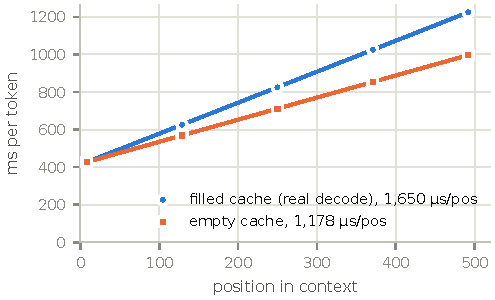
\includegraphics[width=\linewidth]{fig_position.pdf}
\caption{Cost per token against position, shipped shape, battery; each point averages 12
positions. Filling the KV cache raises the slope by 40\%.}
\label{fig:position}
\end{minipage}\hfill
\begin{minipage}[t]{0.49\linewidth}\centering
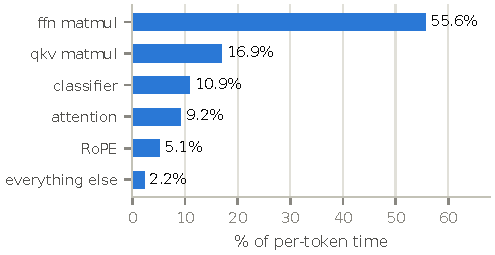
\includegraphics[width=\linewidth]{fig_stages.pdf}
\caption{Where one token's 428.8\,ms goes, shipped shape, positions 3 to 14, battery. Attention's
share grows with position.}
\label{fig:stages}
\end{minipage}
\end{figure}

\textbf{Where the time goes.} Timing each stage of a token at positions 3 to 14 accounts for all but
0.28\% of the measured 428.8\,ms (Figure~\ref{fig:stages}). Matrix products take 83.9\% of it: the
feed-forward block 56.7\%, the query, key and value projections 16.5\% and the classifier 10.6\%.
Attention takes 9.0\% and rotary embeddings 5.0\%. The parts agree with each other within the same
run and at the same positions: the fixed stages are within 0.15\% of the depth intercept, the
per-layer stages within 0.31\% of the depth slope, and all stages together within 0.03\% of the
position model at their mean position.

\textbf{Prediction.} Adding up the position model over the positions of a real decode predicts the
decode time of a run it was not fitted to, recorded by a different program: 18.53\,s predicted
against 18.60\,s measured for 35 tokens at positions 53 to 87 ($-0.4\%$), a decode speed of 1.88
tokens/s. This is one run of one prompt, so it checks the per-token model, not a varied workload,
and it excludes prefill (processing the prompt before the first output token), which took 24.3\,s
for 53 tokens. Three decode runs on the engine before the fix of Section~\ref{sec:defect} ranged
from 1.920 to 1.923 tokens/s.

\textbf{An empty cache measures a cheaper computation.} Our first benchmark reached position $p$ by
jumping there, leaving the cache rows below $p$ unwritten and therefore zero. With the input token held fixed, so that the cache contents are the
only difference, filling the cache raised the fitted cost
per position by 40\%, from 1,182 to 1,651\,\textmu s, with the intercept within 1.6\%. The likely
reason is that without an FPU every multiply-add and exponential in attention is a software routine,
and those routines take shortcuts when an operand is zero; we have not checked this at the
instruction level. The empty-cache model under-predicts the decode run above by 5.3\%.

% ==================================================================================================
\section{Memory and Speed Limits}
\label{sec:frontier}

\textbf{Memory.} Right after a reset, the largest single block an application can allocate is
21.53\,MiB. The checkpoint is one block, but it is not the only constraint: the engine also holds an
fp32 KV cache of $2 \cdot L \cdot \mathrm{context} \cdot \mathrm{width} \cdot 4$ bytes. At the
shipped shape the cache is 8.25\,MiB, 43\% of the 19.34\,MiB that checkpoint and cache take together
(Figure~\ref{fig:memory}). The next width in the same layout, 440 with ten heads and 16.6M parameters, needs
27.19\,MiB for the two and fails to load on the device, although its 16.87\,MiB checkpoint alone
would fit in one block. A 12.2M-parameter model of width 384, in a group-32 layout, did load, with
22.10\,MiB in its two blocks. For six layers, a 512-token context and an fp32 cache, the limit
therefore lies between 12.2M and 16.6M parameters, and because the cache grows linearly with context
length, context and parameters trade off
directly.

The largest block also depends on what the device did recently: after a program failed inside the
loader it was 5.02\,MiB until the calculator was reset, while four load-and-free cycles of the shipped model left it
unchanged to the byte, so the loss comes from the crash, not from fragmentation.

\begin{figure}[t]
\centering
\begin{minipage}[t]{0.49\linewidth}\centering
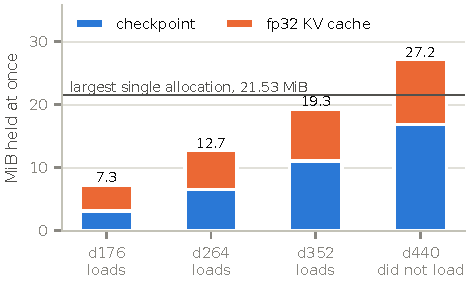
\includegraphics[width=\linewidth]{fig_memory.pdf}
\caption{Checkpoint and fp32 KV cache per width (six layers, context 512), and whether the model
loaded. The shaded band is where the limit on the two-block total must lie; width 384 is a group-32
layout. The largest single block right after a reset was 21.53\,MiB.}
\label{fig:memory}
\end{minipage}\hfill
\begin{minipage}[t]{0.49\linewidth}\centering
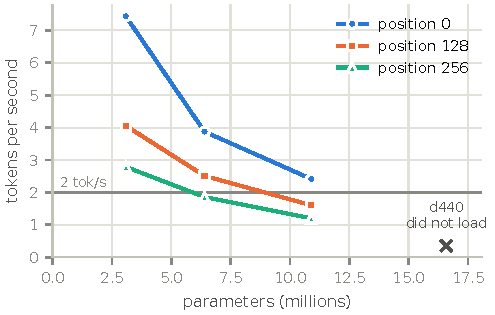
\includegraphics[width=\linewidth]{fig_frontier.pdf}
\caption{Speed against parameters, battery, filled cache, feed-forward width padded to a multiple of
88. Solid: positions 11--18 and 259--266 (Table~\ref{tab:frontier}); dashed: position 128,
interpolated. Widths 176 and 264 use random weights.}
\label{fig:frontier}
\end{minipage}
\end{figure}

\textbf{Speed.} Timing each width with a filled cache gives Table~\ref{tab:frontier} and
Figure~\ref{fig:frontier}. Over positions 11 to 18 the largest tested configuration that reaches 2
tokens/s is the shipped 10.9M; at position 128, by linear interpolation between the two measured
windows, it is the 6.4M width (about 2.5 tokens/s); over positions 259 to 266 it is 3.1M. At short
context, memory and speed set the same limit on width.

\begin{table}[t]
\caption{Speed and memory by width on battery, filled KV cache, context 512. Tokens/s averaged over positions
11--18 and 259--266. Widths 176 and 264 use random weights; the feed-forward width of every file is
padded to a multiple of 88, as in the shipped one.}
\label{tab:frontier}
\centering\small
\begin{tabular}{rrrrr}
\toprule
width & params & file + KV & 11--18 & 259--266 \\
\midrule
176 & 3.09M & 7.26\,MiB & 6.82 & 2.72 \\
264 (6 heads) & 6.40M & 12.70\,MiB & 3.64 & 1.82 \\
352 & 10.90M & 19.34\,MiB & 2.27 & 1.18 \\
440 (10 heads) & 16.59M & 27.19\,MiB & \multicolumn{2}{c}{does not fit} \\
\bottomrule
\end{tabular}
\end{table}

\textbf{When random weights are valid.} Timing untrained widths with random weights is sound only if
decode time does not depend on the weights' values. At width 352 a random-weight model and the
trained one differ by 1.2\% over positions 11 to 18 and by 3.9\% over 259 to 266, consistent with software floating point's
data-dependent timing. The threshold results above would
survive differences of that size, but the comparison does not bound weight-dependent variation at
the other widths.

\textbf{Flash as the alternative.} Streaming weights from flash, as CasioLLM does
\citep{samilososami2026casiollm}, avoids the RAM limit, but on this calculator sequential flash reads
run at about a forty-eighth of the DRAM read speed, so we keep the model in memory.

% ==================================================================================================
\section{Limitations}
\label{sec:limits}

\textbf{The evaluation is synthetic.} Every item except the 2,000 out-of-scope questions, including the fresh ones
of Section~\ref{sec:e2e}, comes from the generators that produced the training documents and uses the store's own
symbols, with values the model has not seen. How often students' own wording and notation lead to a
confident choice is not measured, almost every call in the evaluation
is to \tok{eval}, one of the seven tools, and we do not report perplexity. The model cannot judge whether a relation fits
(Section~\ref{sec:quality}), so a question answered with the wrong relation, such as the ambiguous
resistance question, gets a confident wrong answer.

\textbf{One device, and few repeats.} All timings come from one calculator. On the shipped engine the decode speed was measured once, as were most other timing cells.
Appendix~\ref{app:ladder} compares only two widths.

\textbf{Explanations are scored for form, not truth.} Whether an explanation's physics is correct is
not measured, and the explanation training text has not been reviewed by a person
(Section~\ref{sec:data}).

% ==================================================================================================
\section{Conclusion}
\label{sec:conclusion}

Given the right relation, a 10.9M-parameter model that never computes is right on 96.7\% of fully
specified physics problems on the calculator's own decoder, and its wrong answers are copying
errors. A rule-based path through the same
runtime with no model answers all of these problems correctly, and behind the application's
own selector it is still right more often and wrong less often, while the model declines more
reliably when selection goes wrong. Each step that brought our evaluation closer to the deployed system changed its result: one exposed an engine defect that a
host--calculator comparison could not see, and the last showed that most of the original
system's accuracy was lost before the model ran, in a step with no neural network. On hardware this
limited, the evaluation worth reporting is the one that runs the device's own code, end to end, and
counts wrong answers and declines as well as right ones.

\label{endofmain}

% --------------------------------------------------------------------------------------------------
\section*{Broader Impact Statement}

A physics assistant on a device allowed in some examinations could be used to answer examination
questions. The system chooses the relation itself when it is confident and declines otherwise, but a
student can still get a confident wrong answer when a question is ambiguous or the chosen relation
does not apply, which the model cannot detect. The explanation texts it learned from were drafted by
an AI model and have not been reviewed by a person. The store, the corpus and the weights will be
released, so an institution can inspect what the assistant contains and decide whether to allow it.

\section*{Statements and Declarations}

\begin{itemize}
\setlength{\itemsep}{1pt}
\item \textbf{Funding.} No external funding was received for this work.\ifdeanonymized{} The author
funded the project personally.\fi
\item \textbf{Competing interests.} \Theauthor{} \ifdeanonymized declares\else declare\fi{} no
competing interests.
\item \textbf{Data availability.} The record store, the training corpus, the trained weights, and the
device logs and results behind every table and figure will be released with the final version of
this paper. The corpus, the store and the weights will be released under CC BY-NC-SA~4.0, following the licenses of the OpenStax source text.\ifdeanonymized\else{} A video of the calculator in use
(Appendix~\ref{app:device}) is in the supplementary material.\fi
\item \textbf{Code availability.} The code, including the calculator application, the inference
engine, the corpus generator and the evaluation harness, will be released with the final version of
this paper, under the MIT License for the code written for this work and the Mozilla Public
License~1.1 for the loader derived from Ndless.
\ifdeanonymized
\item \textbf{Author contributions.} The author initiated and directed the project, oversaw all
agentic workflows, checked the results, carried out the measurements on the calculator, edited the
text and personally funded the project. The author takes full responsibility for the work.
\fi
\item \textbf{Use of AI tools.} Anthropic's Claude models, mainly Claude Opus~5 and Claude Opus~5.5,
used through the Claude Code command-line interface, wrote most of the software and experiment
tooling, ran most of the host-side experiments and analyses, and drafted the text. The explanation documents in the training data were also drafted by these models (Section~\ref{sec:data}).
\Theauthor{} directed the work, carried out the
measurements on the calculator, checked the results and chose what to report.
\item \textbf{Trademarks.} TI-Nspire is a trademark of Texas Instruments, and Casio and fx-CG50 are
trademarks of Casio Computer Co.; this work is not affiliated with or endorsed by either company.
\end{itemize}

\bibliography{references}
\bibliographystyle{tmlr}

\appendix
% ==================================================================================================
\section{Two Model Widths}
\label{app:ladder}

We trained a 3.1M-parameter model of width 176 exactly as we trained one of width 352: the same
corpus version and tokenizer, six layers, eight heads, 8,000 steps at batch 24 and the same
learning-rate schedule, with two training seeds at each width. Width is the only difference. The two
widths were chosen under the group-88 layout, so the comparison has two points and we fit nothing through
them. All four models are scored as in Section~\ref{sec:quality}, with the relation
supplied, on the calculator's decoder with a group size of 16, which divides every row at both
widths. The shipped layout differs from group 16 by at most 1.7 points on the shipped model.

\begin{table}[t]
\caption{The two widths on the calculator's decoder (int8, run on the host), group 16, greedy,
relation supplied. Each cell is the percentage of items passed by one training seed (s1, s2); the
change is between the two-seed means, in points. Items per set as in Table~\ref{tab:quality}. The
explanation row is the format check.}
\label{tab:ladder}
\centering\small
\setlength{\tabcolsep}{5pt}
\begin{tabular}{@{}lrrrrr@{}}
\toprule
 & \multicolumn{2}{c}{3.1M} & \multicolumn{2}{c}{10.9M} & \\
\cmidrule(lr){2-3}\cmidrule(lr){4-5}
item set & s1 & s2 & s1 & s2 & change \\
\midrule
decline: value withheld & 99.2 & 100.0 & 99.2 & 100.0 & 0.0 \\
decline: no values & 100.0 & 100.0 & 100.0 & 100.0 & 0.0 \\
right: values given & 65.0 & 83.3 & 95.0 & 92.5 & $-19.6$ \\
right: named by symbol & 70.8 & 77.5 & 99.2 & 98.3 & $-24.6$ \\
right: named in words & 75.0 & 80.8 & 96.7 & 95.8 & $-18.3$ \\
right: irrelevant value added & 41.7 & 55.8 & 63.3 & 52.5 & $-9.2$ \\
explanation (format) & 64.4 & 52.9 & 93.1 & 93.1 & $-34.5$ \\
decline: relation does not apply & 0.0 & 0.0 & 0.0 & 15.8 & $-7.9$ \\
\bottomrule
\end{tabular}
\end{table}

\textbf{Declining is unchanged.} Declining when the prompt names a missing value is not affected by the 3.5-fold
reduction in parameters: 99.6\% at both widths, and 100\% when no values are given at all
(Table~\ref{tab:ladder}).

\textbf{Numeric answers get worse, in the call.} Accuracy falls by 18 to 25 points on the three
answerable sets, from 93.8\% to 74.2\% when every value is given. The loss is in the call. Calls
built with a wrong value are 1.7\% and 5.0\% of items at width 352 and 32.5\% and 13.3\% at width
176, while failures of the strict
criterion stay between 8\% and 18\% at both widths. With an extra value
present both widths do poorly and the gap narrows to 9 points.

\textbf{Explanation format drops the most, and judging fit fails at both widths.} Passing the
explanation format check falls from 93.1\% to 58.6\%, the largest drop in the table. Declining a relation that does not apply is at or near zero throughout;
the one exception, 15.8\%, comes from the second seed at width 352, which also scored highest on this
set under earlier scoring, and we read it as seed variation rather than
a capability.

One description consistent with these numbers is that the accuracy drop grows with how much the model
must produce beyond what the prompt already contains: a one-line refusal, a call that copies several
values, a paragraph of text. We did not vary that amount with the task held fixed, so it is a
description, not a mechanism. The width-176 seeds differ by up to 18 points, and two seeds are not a
variance estimate; equal optimizer steps do not hold convergence constant either (final losses 0.963
and 0.952 at width 176, 0.799 and 0.787 at 352). Predictions we registered before training named an
item set we later found measures declining, scored by a harness we later replaced
(Section~\ref{sec:harness}), so this experiment is not a test of them.

% ==================================================================================================
\clearpage
\makeatletter\setlength{\@fptop}{0pt}\makeatother   % a page holding only figures starts at the top
\section{The Calculator in Use}
\label{app:device}

Figure~\ref{fig:device} shows three frames from a video of the calculator answering the question of
Figure~\ref{fig:exchange}, filmed in one take on battery with no cable attached. ChatTLM Setup, opened
after the reset button on the back of the calculator was pressed, installs the loader and closes, and the home screen reports it (a). The question was
then typed on the keypad, whose letter keys are in alphabetical order, and entered. This time the
application chose the relation itself, and it printed the same answer as in
Figure~\ref{fig:exchange}, complete about 59\,s after the question was entered (b, c). That time is
read from the video; unlike the 52.0\,s of Figure~\ref{fig:exchange}, it includes choosing the
relation, building the prompt and tokenizing it. \ifdeanonymized The video will be released with the
code.\else The video, unedited apart from re-encoding, is in the supplementary material.\fi

\begin{figure}[h]
\centering
\begin{tabular}{@{}c@{\hspace{1em}}c@{\hspace{1em}}c@{}}
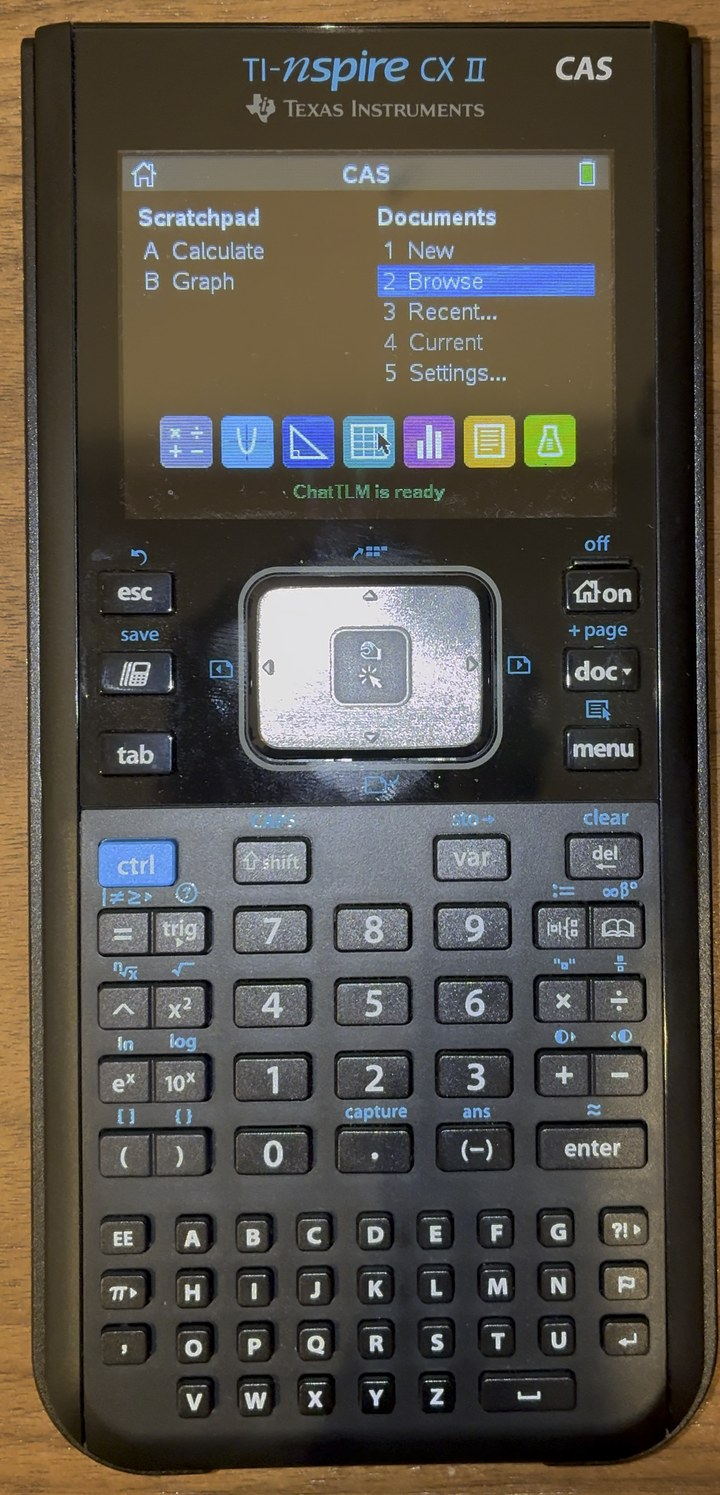
\includegraphics[height=6.4cm]{photo_ready.jpg} &
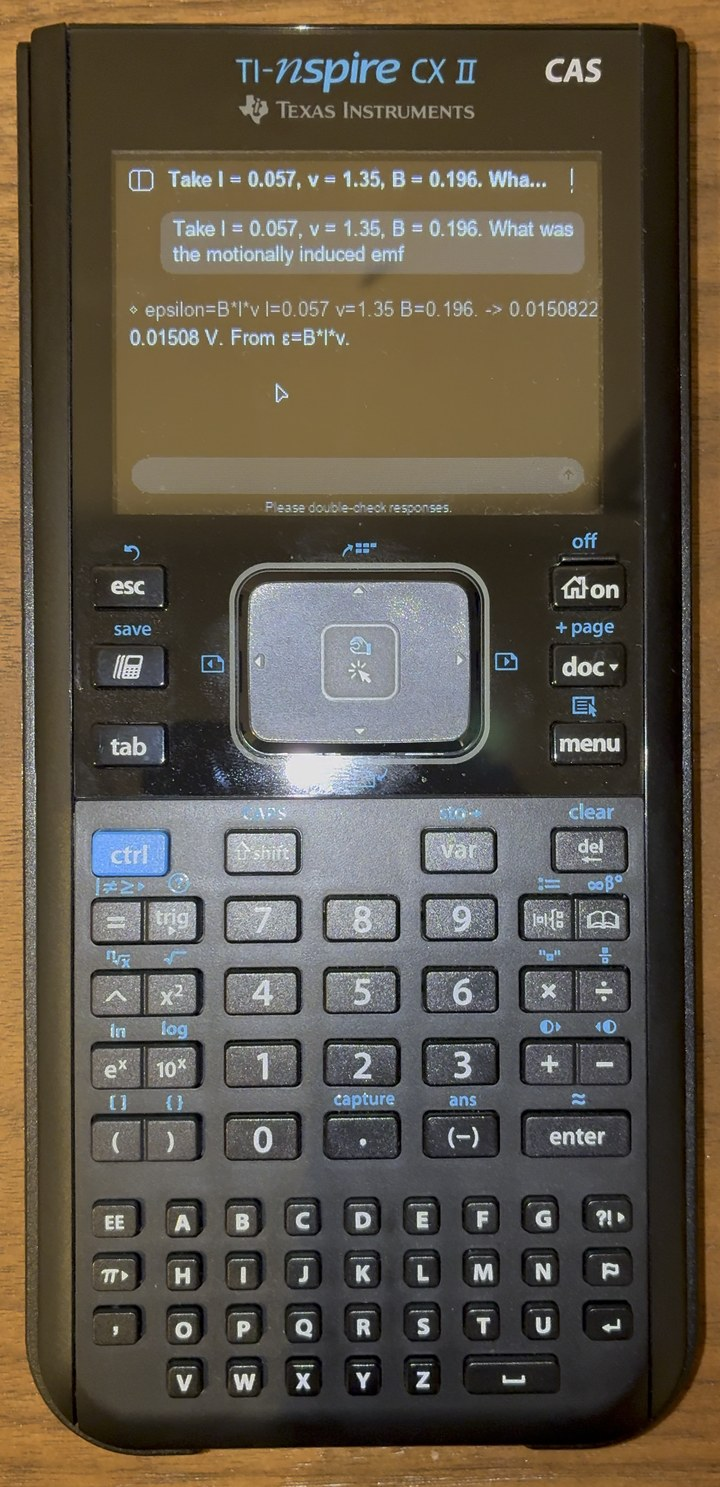
\includegraphics[height=6.4cm]{photo_answer.jpg} &
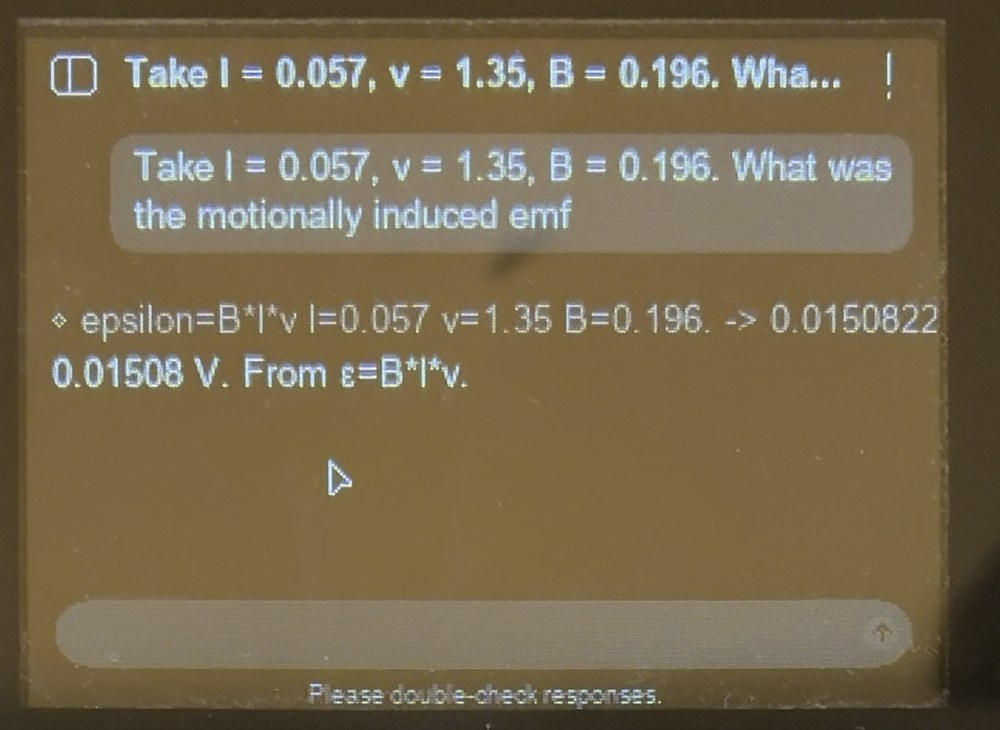
\includegraphics[height=6.4cm]{photo_screen.jpg} \\
\small (a) & \small (b) & \small (c)
\end{tabular}
\caption{Frames from the video, cropped and scaled but not retouched. (a)~The home screen after ChatTLM
Setup has run; the green line reads ``ChatTLM is ready'' and the battery symbol is at the top right.
(b)~The finished answer. (c)~The screen of (b), enlarged: the question, the relation the application
chose with the values it read and the result of the call (\tok{epsilon=B*l*v l=0.057 v=1.35
B=0.196.\ -> 0.0150822}, with the stray period noted under Figure~\ref{fig:exchange}), and the answer.}
\label{fig:device}
\end{figure}

Figure~\ref{fig:screens} shows four screens drawn by the application's own drawing code, compiled for
a computer, at the calculator's 320$\times$240 pixels. The application chooses the relation and
builds the line above each answer exactly as it does on the calculator, and each answer is the output
of the calculator's decoder run on the host, which matches the calculator token for token
(Section~\ref{sec:parity}). Screen (b) is the one filmed in Figure~\ref{fig:device}c.

\begin{figure}[h]
\centering
\begin{tabular}{@{}c@{\hspace{1.2em}}c@{}}

\includegraphics[width=0.44\linewidth]{screen_start.png} &
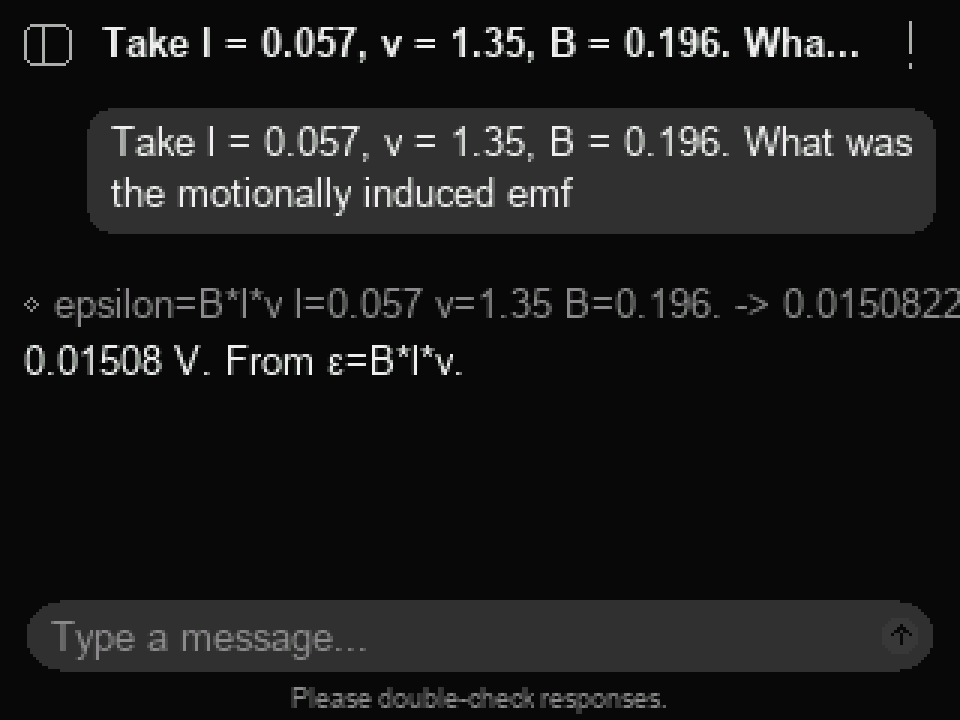
\includegraphics[width=0.44\linewidth]{screen_emf.png} \\
\small (a) & \small (b) \\[4pt]
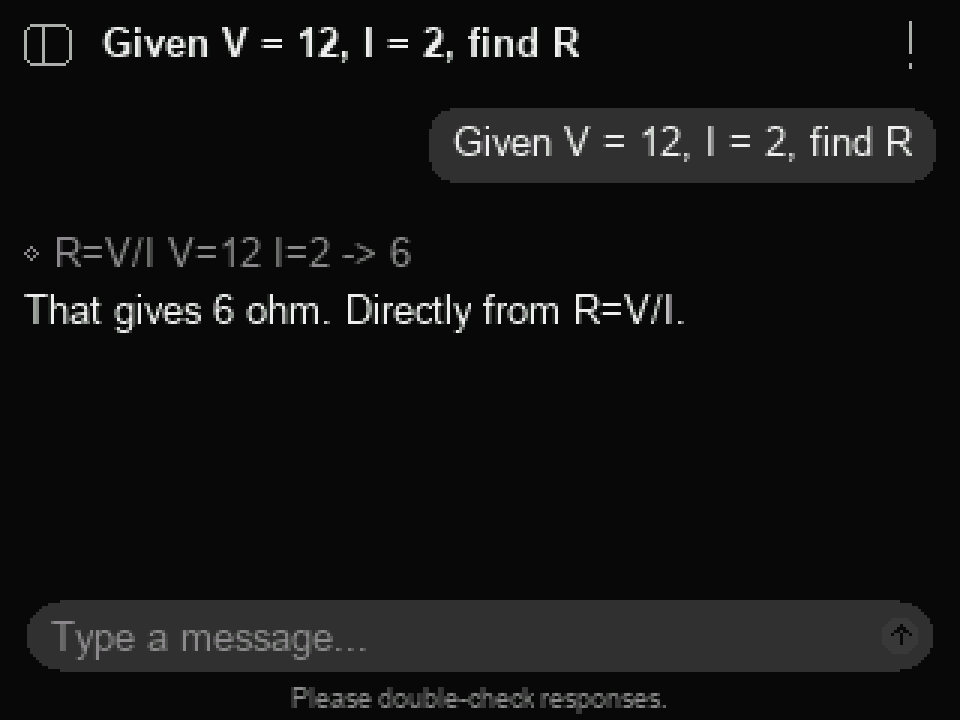
\includegraphics[width=0.44\linewidth]{screen_symbol.png} &

\includegraphics[width=0.44\linewidth]{screen_decline.png} \\
\small (c) & \small (d)
\end{tabular}
\caption{Screens drawn by the application's own code, in the dark theme the calculator was using when
it was filmed (the theme follows the clock). (a)~The start screen. (b)~The question of
Figure~\ref{fig:device}, as it was typed. (c)~A question that names its values by symbol. (d)~A
question no record answers, which the application declines. Above each answer is the relation the
application chose (``none'' in (d)), with the values it read and the result of the call.}
\label{fig:screens}
\end{figure}

\end{document}
